% Template for ICASSP-2020 paper; to be used with:
%          spconf.sty  - ICASSP/ICIP LaTeX style file, and
%          IEEEbib.bst - IEEE bibliography style file.
% --------------------------------------------------------------------------
\documentclass{article}
\usepackage{spconf,amsmath}
\usepackage{graphicx}
\usepackage{multirow}
\usepackage{array}
\usepackage{subfig}

\usepackage[dvipsnames]{xcolor}
\definecolor{mypink1}{rgb}{0.858, 0.188, 0.478}
\definecolor{mypink2}{RGB}{219, 48, 122}
\definecolor{mypink3}{cmyk}{0, 0.7808, 0.4429, 0.1412}
\definecolor{mygray}{gray}{0.6}

\usepackage{amsmath}  %use \therefore
\usepackage{amssymb} %use \therefore

\usepackage{tikz} %use circle{1}
\newcommand*\circled[1]{\tikz[baseline=(char.base)]{
		\node[shape=circle,draw,inner sep=0.4pt] (char) {#1};}}

\usepackage[ruled,vlined]{algorithm2e} %use Algorithm structure

% Example definitions.
% --------------------
\def\x{{\mathbf x}}
\def\L{{\cal L}}

%---
\usepackage{CJKutf8}  %use Chinese fonds

%--- highlight
\usepackage{color,soul}
%---
\usepackage{listings} %can insert Python


% Title.
% ------
\title{Camera Calibration: Pinhole Model(intrinsic parameters)+Distortion Elimination(extrinsic parameters)+Chess Board Parameter Regress(the solution)}
%
% Single address.
% ---------------
\name{Bo Wu$^{\star \dagger}$ \qquad }

			\address{$^{\star}$data for the demo: OpenCV Official\\
			    $^{\dagger}$ Toronto, ON, CA on July 06, 2020 }

%\name{Shuai Zheng\textsuperscript{1,2}, Xiao-Ping Zhang\textsuperscript{2}, Jian Chen\textsuperscript{1}, Yonghong Kuo\textsuperscript{1}}
%\address{\textsuperscript{1}School of Telecommunications Engineering, Xidian University, China \\ \textsuperscript{2}Department of Electrical and Computer Engineering, Ryerson University, Canada}
%
% For example:
% ------------
%\address{School\\
%	Department\\
%	Address}
%
% Two addresses (uncomment and modify for two-address case).
% ----------------------------------------------------------
%\twoauthors
%  {A. Author-one, B. Author-two\sthanks{Thanks to XYZ agency for funding.}}
%	{School A-B\\
%	Department A-B\\
%	Address A-B}
%  {C. Author-three, D. Author-four\sthanks{The fourth author performed the work
%	while at ...}}
%	{School C-D\\
%	Department C-D\\
%	Address C-D}
%
\begin{document}
\ninept
%
\onecolumn
\maketitle
%
\begin{abstract}
TBD
\subitem{* TBD}
\subitem{* TBD}
\end{abstract}
%
\begin{keywords}
Camera Calibration
\end{keywords}

%%% \onecolumn
%%%%% \twocolumn %or don't need it, it will become two columns automatically

% \vfill\pagebreak

%--------------------------------------------------------------------------------%
%--------------------------------------------------------------------------------%
\section{Background}
\label{sec: section_Background}

TBD
	\begin{enumerate}
		\item TBD;
		\item TBD;
		\item TBD.
	\end{enumerate}
	
TBD

%--------------------------------------------------------------------------------%
%--------------------------------------------------------------------------------%
\section{Goal}
\label{sec:CC_goal}
\hl{The ultimate goal of camera calibration is to undistort images based off the intrinsic and extrinsic properties of a camera.}
% =======
% FIG. 01 Pinhole Camera Model
% =======
\begin{figure}[!t]
	\centering
	\includegraphics[height=4.1in,width=5.0 in]{./img_cur/pinhole_camera_model.jpeg}
	\caption{Pinhole Camera Model.}
	\vspace{-1.0em}
	\label{fig_Pinhole}
\end{figure}

%--------------------------------------------------------------------------------%
%--------------------------------------------------------------------------------%
\begin{CJK}{UTF8}{gkai}  
\section{Camera Calibration: 针孔(-内参) + 消畸(-外参) + 标定板参数拟合(-solution)}
\label{sec:previous_notes_on_cc_BW}
	
\subsection{CC在做什么?}	
	\begin{itemize}
		\item [1.] 由像素坐标到世界坐标的相互切换。(基于针孔模型,4个内参)
		\item [2.] 需要借助图像坐标、相机坐标作为中间辅助。
		\item [3.] 除去针孔模型,还需要考虑相机的径向畸变(radial distortion)和切向畸变(tangential distortion)。(5个外参)
		\item [4.] 用标定板进行参数拟合的时候还得多计算旋转矩阵$R_{B2C}$和平移矩阵$T_{B2C}$。(B2C: Board标定板 to Camera)
	\end{itemize}
	
\subsection{Camera Calibration--@BW notes}	
\label{ssec: camera_calibration_notes_BW}
	% =======
	% FIG. 02 BW-previous notes
	% =======
	\begin{figure}[!t]
		\centering
		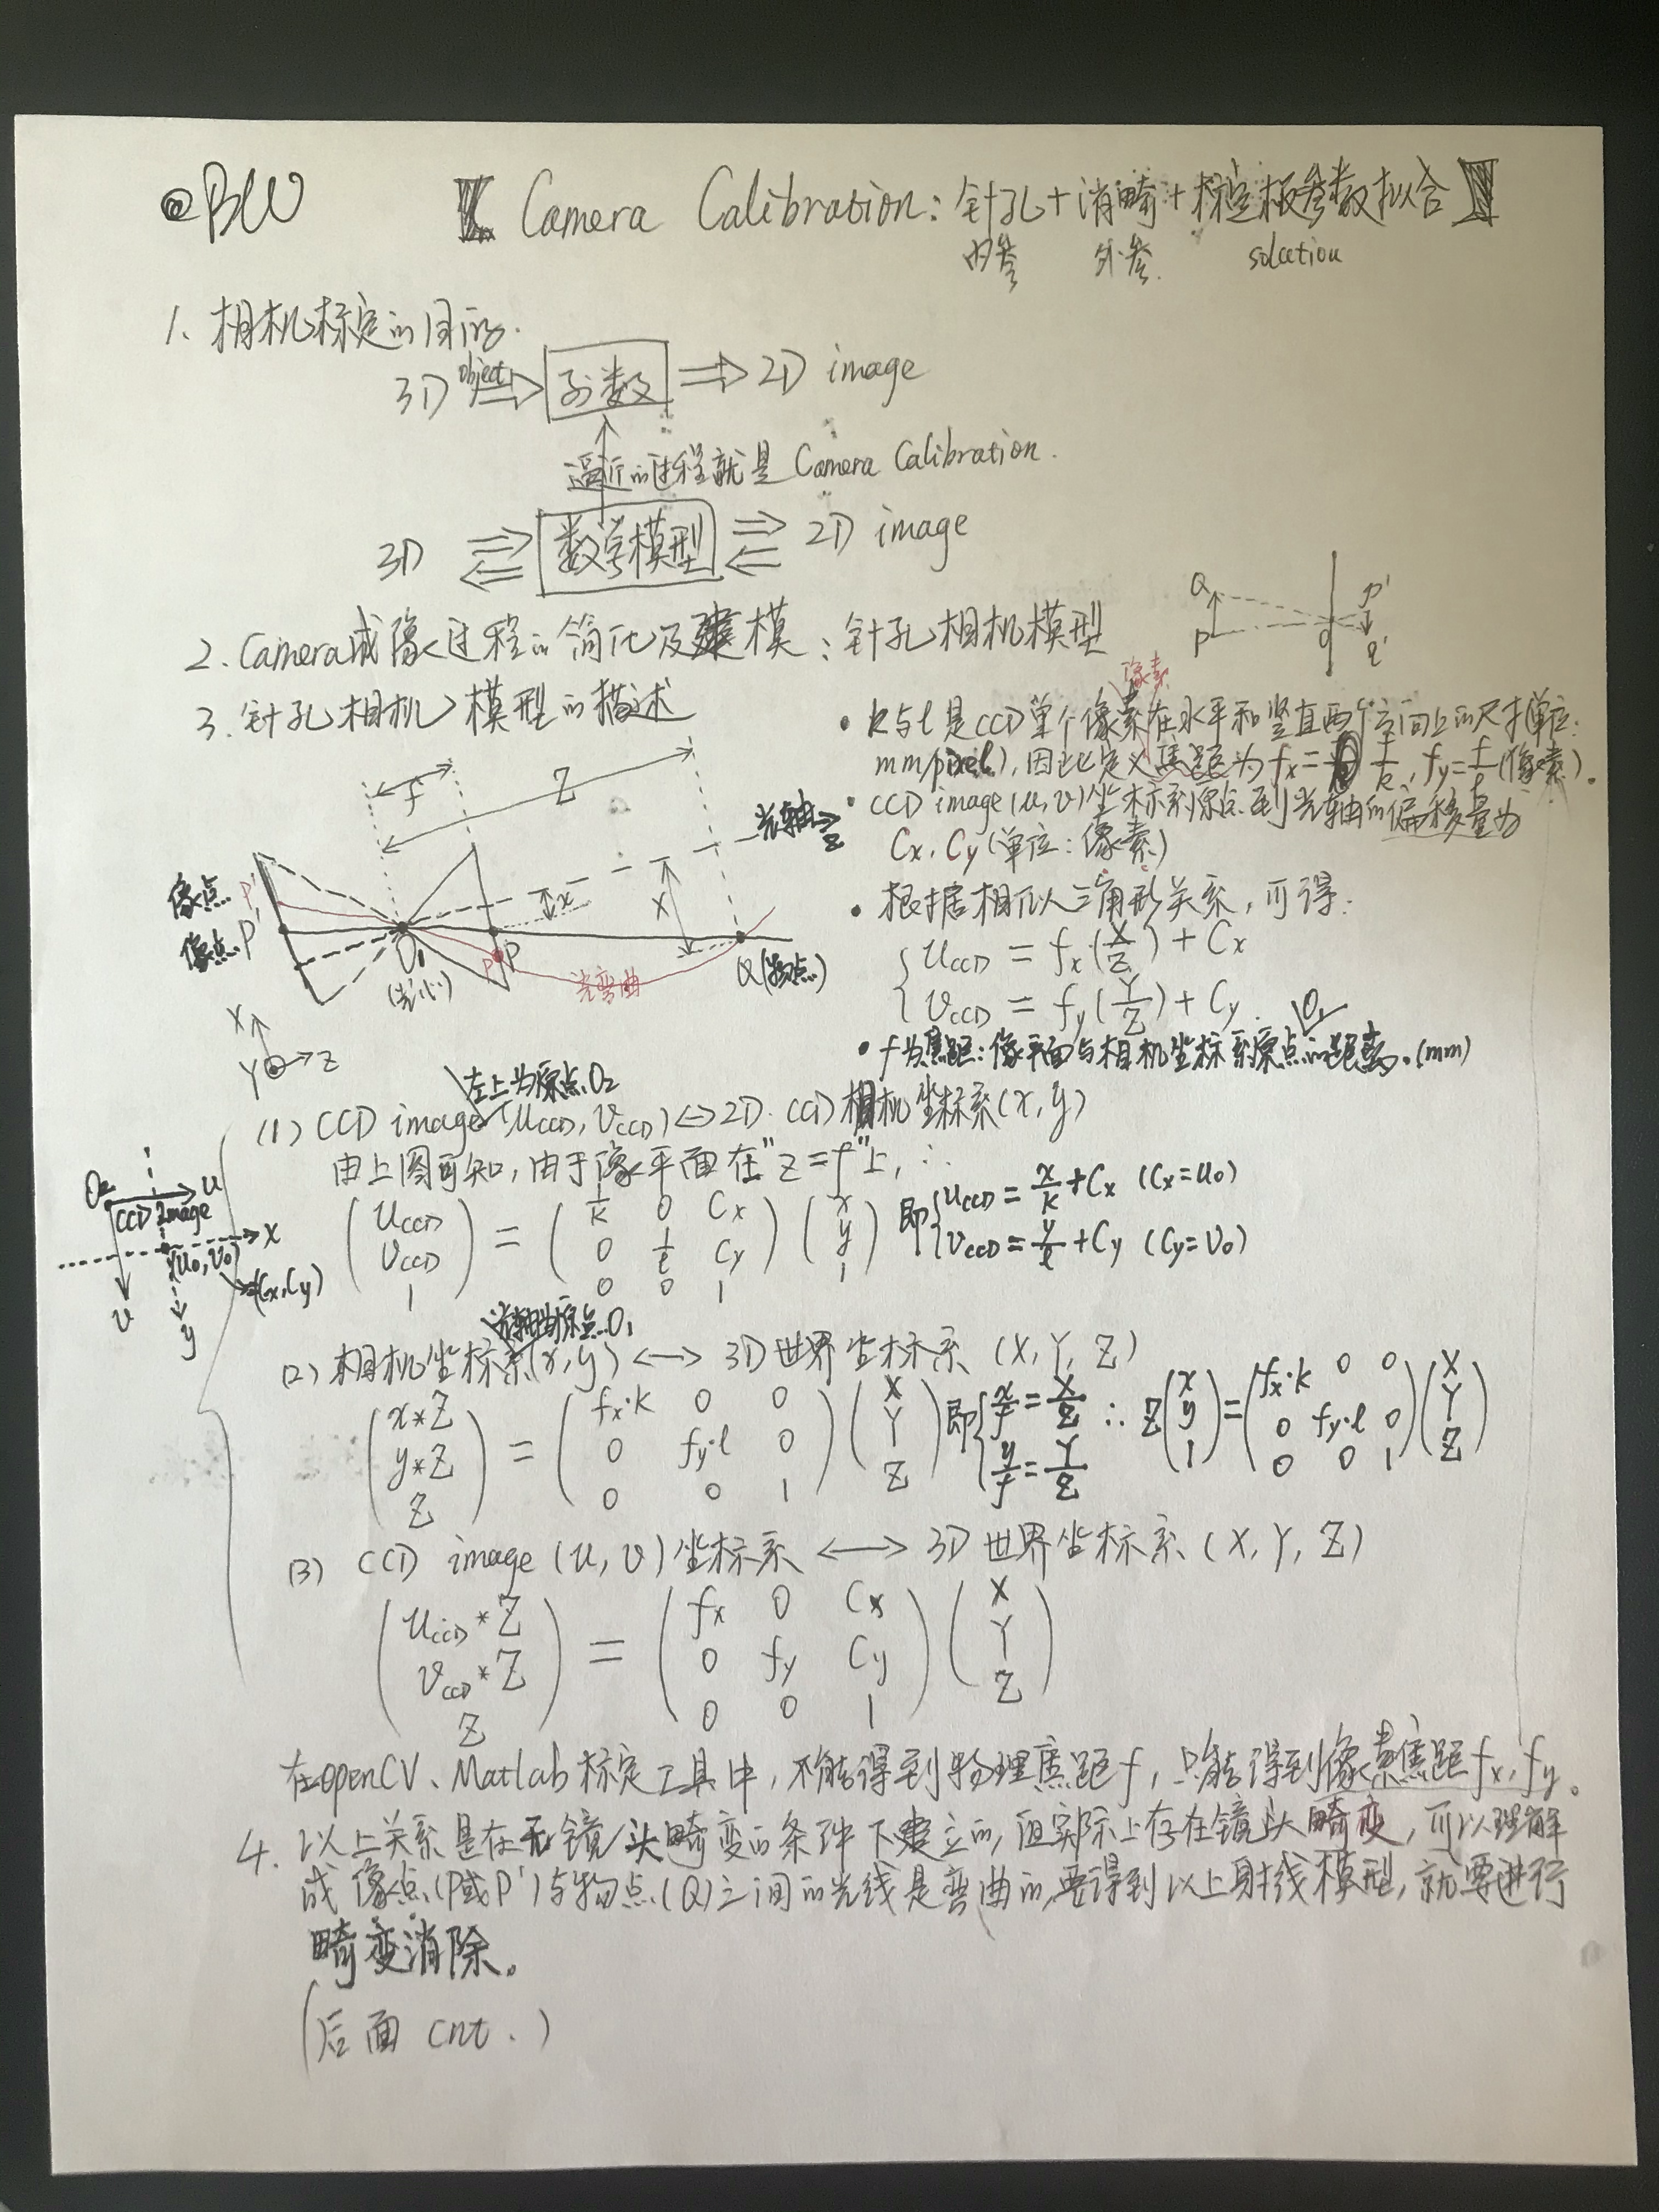
\includegraphics[height=8.5in,width=6.0 in]{./img_cur/camera_calibration_1over2.png}
		\caption{摄像头标定个人之前笔记之Page 1/2.}
		\vspace{-1.0em}
		\label{fig_CameraCalibration_1over2_BW}
	\end{figure}

	\begin{figure}[!t]
		\centering
		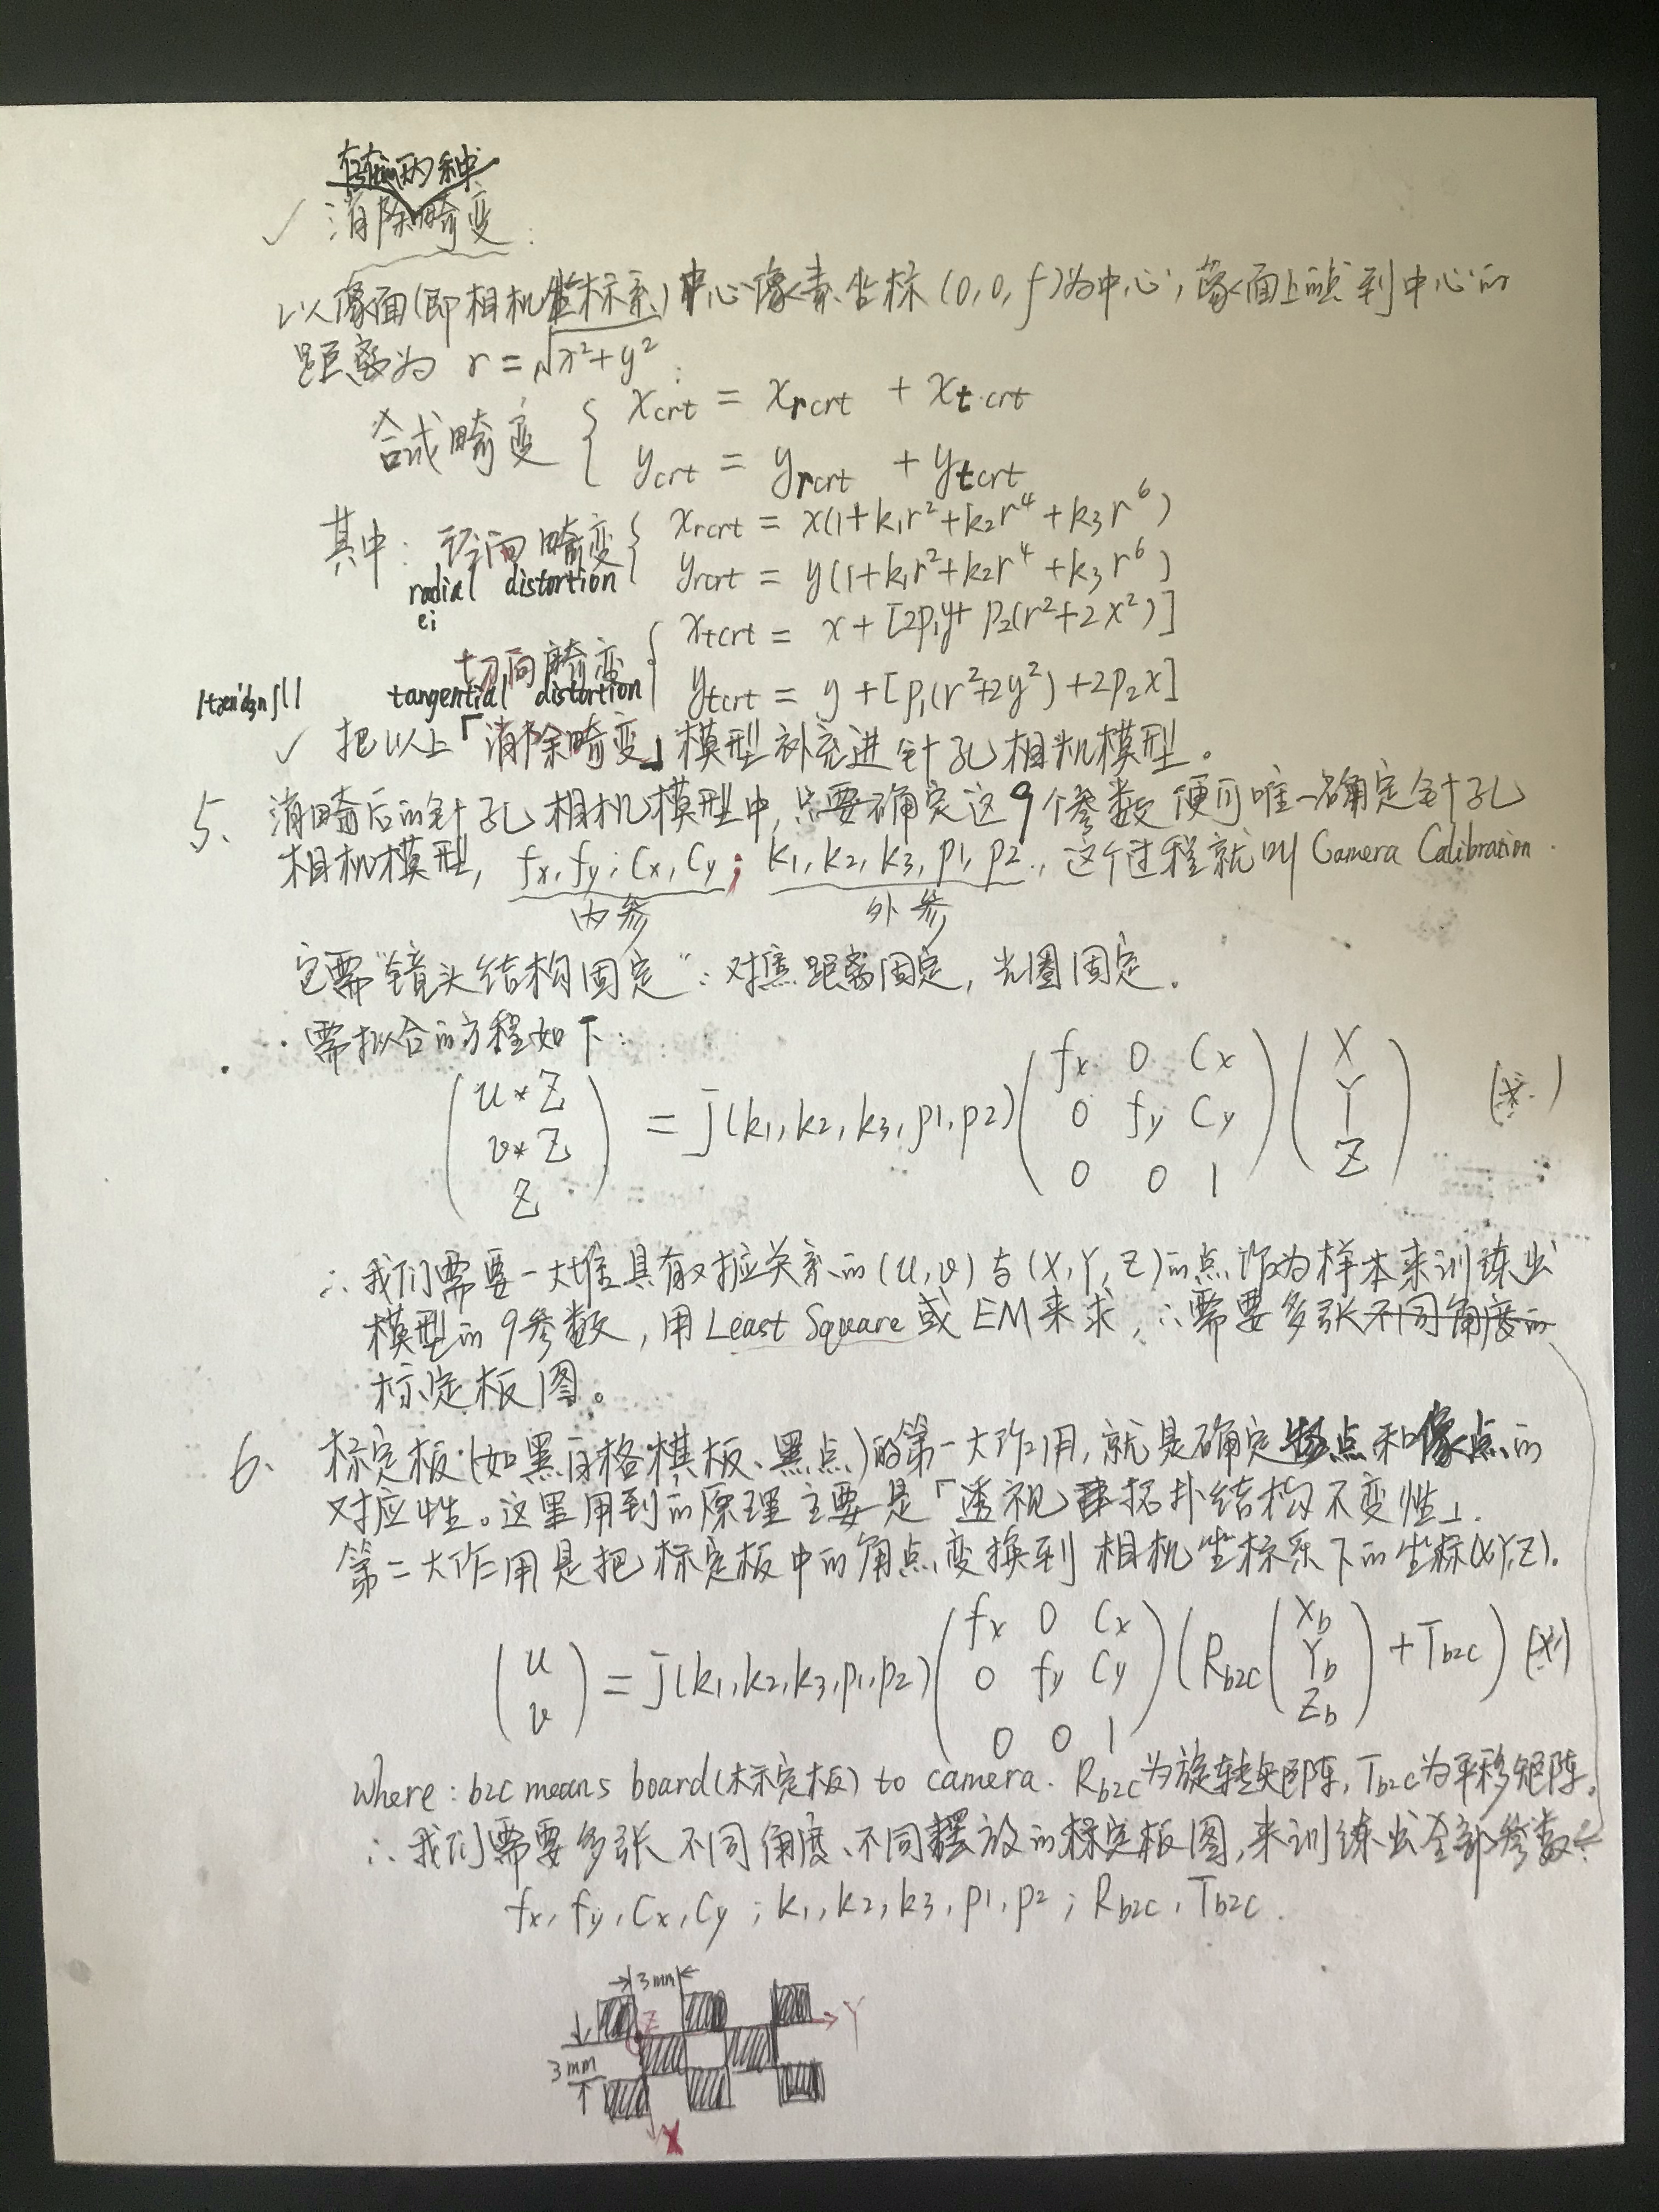
\includegraphics[height=8.5in,width=6.0 in]{./img_cur/camera_calibration_2over2.png} 
		\caption{摄像头标定个人之前笔记之Page 2/2.}
		\vspace{-1.0em}
		\label{fig_CameraCalibration_2over2_BW}
	\end{figure}
\end{CJK}

%--------------------------------------------------------------------------------%
%--------------------------------------------------------------------------------%
\section{Math Equations of Above Section}
\label{sec:Math_Equ_conclusion}
I've made some corrections of my previous notes here, refered from \cite{ref_Four_Coordinates} and \cite{ref_OpenCV_camera_calibration}.

\subsection{Correction I-Four Coordinates}
\label{ssec:math_Correction_I}
$\bigstar$ \hl{\textbf{BW: There are 4 coordinates not 3.}}
\begin{itemize}
	\item [1.] \textbf{Pixel Coordinates}: $(u,v)$. As shown in Fig. \ref{fig_Pinhole}, its origin (u=0,v=0) is at its upper-left corner.
	\item [2.] \textbf{Image Coordinates}: $(x,y)$. As shown in Fig. \ref{fig_Pinhole}, its origin (x=0,y=0) is at the image center.
	\item [3.] \textbf{Camera Coordinates}: $(X_C,Y_C,Z_C)$. As shown in Fig. \ref{fig_Pinhole}, its origin $(X_C=0,Y_C=0,Z_C=0)$ is at its optical point $F_C$.
	\item [4.] \textbf{World Coordinates}: $(X,Y,Z)$. As shown in Fig. \ref{fig_Pinhole}, often its origin (X=0,Y=0,Z=0) is at the same with Camera Coordinates.
\end{itemize}

Their relations are as follows. \begin{itemize}
	\item [$\bigstar$] \hl{Pixel to Image:}
		\begin{equation}
			\begin{array}{l}
				u = \frac{x}{k} + c_x \\
				v = \frac{y}{l} + c_y
			\end{array}
			\label{Eq_Pixel2Image}
		\end{equation}
		where $k$, $l$ represent the physical size of one pixel in image array, respectively (unit: mm/pixel); $c_x$, $c_y$ denote the coordinates of [the Origin of Image Coordinates] at the Pixel Coordinates. It also can be written in vector multiplication form as below. 
		
		\begin{equation}
			\left[\begin{array}{l}
			u \\
			v \\
			1
			\end{array}\right]= \left[\begin{array}{lll}
			\frac{1}{k} & 0 			& c_{x} \\
			0 			& \frac{1}{l}	& c_{y} \\
			0  			& 0 			   & 1
			\end{array}\right]\left[\begin{array}{l}
			x \\
			y \\
			1
			\end{array}\right]			
			\label{Eq_Pixel2Image_vector_format}
		\end{equation}
		
	\item [$\bigstar$] \hl{Image to Camera:}
		\begin{equation}
			\begin{array}{l}
				\frac{x}{f} = \frac{X_C}{Z_C}\\
				\frac{y}{f} = \frac{Y_C}{Z_C}
			\end{array}
			\label{Eq_Image2Camera}
		\end{equation}
		where $f$ is the focal length, a.k.a. the distance between the image and the Origin of the Camera Coordinates. And, $f=f_x \cdot k=f_y \cdot l$. Since the calibration tools in OpenCV and Matlab don't provide the calculation of focal length $f$ of the lens but they do provide the computation of pixel-focal-length $f_x$ and $f_y$. We also can reform the above equation to vector format as follows.
		\begin{equation}
		Z_C \left[\begin{array}{l}
		x \\
		y \\
		1
		\end{array}\right]=s\left[\begin{array}{lll}
		f_{x}\cdot k & 0 & 0 \\
		0 & f_{y}\cdot l & 0 \\
		0 & 0 & 1
		\end{array}\right]\left[\begin{array}{l}
		X_C \\
		Y_C \\
		Z_C
		\end{array}\right]			
		\label{Eq_Image2Camera_vector_form}
		\end{equation}
		$\rhd$ Combining (\ref{Eq_Pixel2Image_vector_format}) and (\ref{Eq_Image2Camera_vector_form}), we can get \hl{Pixel to Camera} transformation below.
		\begin{equation}
		Z_C \left[\begin{array}{l}
		u \\
		v \\
		1
		\end{array}\right]=\left[\begin{array}{lll}
		f_{x} & 0 & c_{x} \\
		0 & f_{y} & c_{y} \\
		0 & 0 & 1
		\end{array}\right]\left[\begin{array}{l}
		X_C \\
		Y_C \\
		Z_C
		\end{array}\right]			
		\label{Eq_Pixel2Camera_vector_form}
		\end{equation}
		It's also termed as the $camera\,matrix$:
		  \begin{equation}
		  camera\,matrix = \left[\begin{array}{lll}
		  f_{x} & 0 & c_{x} \\
		  0 & f_{y} & c_{y} \\
		  0 & 0 & 1
		  \end{array}\right]		
		  \label{Eq_camera_matrix}
		  \end{equation}
		$f_x,f_y,c_x,c_y$ are the intrinsic parameters specific to a camera. 
		
	\item [$\bigstar$] \hl{Camera to World:}	
		\begin{equation}
		\left[\begin{array}{l}
		X_C \\
		Y_C \\
		Z_C \\
		1
		\end{array}\right]=\left[\begin{array}{ll}
		R_{3x3} & t_{3x1} \\
		0^T & 1 
		\end{array}\right]\left[\begin{array}{l}
		X \\
		Y \\
		Z \\
		1
		\end{array}\right]			
		\label{Eq_Camera2World_vector_form}
		\end{equation}
		where $R$ denotes the orthogonal rotation matrix with the size of 3x3; $r$ is the 3D translation vector with the size of 3x1.
		
	\item [$\bigstar$] \hl{Pixel to World:}	Combining (\ref{Eq_Pixel2Camera_vector_form}) and (\ref{Eq_Camera2World_vector_form}), we can derive the transformation of Pixel-to-World as follows.
		\begin{equation}
		Z_C \left[\begin{array}{l}
		u \\
		v \\
		1
		\end{array}\right]=\left[\begin{array}{llll}
		f_{x} & 0 & c_{x} &0\\
		0 & f_{y} & c_{y} &0\\
		0 & 0 & 1  &0
		\end{array}\right]\left[\begin{array}{ll}
		R_{3\times 3} & t_{3\times 1} \\
		0^T & 1 
		\end{array}\right]\left[\begin{array}{l}
		X \\
		Y \\
		Z \\
		1
		\end{array}\right] 			
		\label{Eq_Pixel2World_vector_form}
		\end{equation}
\end{itemize}

\subsection{Correction II-Extrinsic and Intrinsic Parameters}
\label{ssec:Correction2_math}
\begin{itemize}
	\item [$\bigstar$] \hl{Extrinsic Parameters:}
	
		Extrinsic parameters corresponds to rotation $R$ and translation vectors $t$ which translates a coordinates of a 3D point to a coordinate system.
		
	\item [$\bigstar$] \hl{Intrinsic Parameters:}	
	
		Intrinsic parameters include information like focal length ($f_x$,$f_y$) and optical centers ($c_x$,$x_y$), a.k.a. the $camera\,matrix$ (\ref{Eq_camera_matrix}). The focal length and optical centers can be used to create a camera matrix, which can be used to remove distortion due to the lenses of a specific camera. The camera matrix is unique to a specific camera, so once calculated, it can be reused on other images taken by the same camera. 
		
\end{itemize}
In short, we need to find four parameters, also known as \textbf{camera matrix} given by:
\begin{equation}
Coefficients\,in\,camera\,matrix = (f_x, f_y, c_x, c_y)
\label{Eq_camera_coeff}
\end{equation}

\subsection{Correction III-Distortion}
\label{ssec:Correction3_math}
Some pinhole cameras introduce significant distortion to images. Two major kinds of distortion are radial distortion and tangential distortion.

\begin{itemize}
	\item [$\bigstar$] \hl{Radial Distortion:}
	
	Radial distortion causes straight lines to appear curved. Radial distortion becomes larger the farther points are from the center of the image. For example, one image is shown in Fig. \ref{fig_Radial_distortion} in which two edges of a chess board are marked with red lines. But, you can see that the border of the chess board is not a straight line and doesn't match with the red line. All the expected straight lines are bulged out.
	\begin{figure}[!t]
		\centering
		\includegraphics[height=4.1in,width=5.0 in]{./img_cur/radial_distortion.jpg}
		\caption{Radial distortion example.}
		\vspace{-1.0em}
		\label{fig_Radial_distortion}
	\end{figure}
	Radial distortion can be represented as follows:
		\begin{equation}
		\begin{array}{l}
			x_{\text {rdistorted}}=x\left(1+k_{1} r^{2}+k_{2} r^{4}+k_{3} r^{6}\right) \\
			y_{\text {rdistorted}}=y\left(1+k_{1} r^{2}+k_{2} r^{4}+k_{3} r^{6}\right)
		\end{array}
		\label{Eq_radial_distortion}
		\end{equation}
		where $r=\sqrt{x^2+y^2}$; $(x,y)$ is the coordinates in Image Coordinates.
	
	\item [$\bigstar$] \hl{Tangential Distortion:}	
	
	Similarly, tangential distortion occurs because the image-taking lense is not aligned perfectly parallel to the imaging plane. So, some areas in the image may look nearer than expected. The amount of tangential distortion can be represented as below:
		\begin{equation}
		\begin{array}{l}
		x_{\text {tdistorted}}=x + \left[2p_{1}xy+p_{2}(r^2+2x^2)\right] \\
		y_{\text {tdistorted}}=y + \left[p_{1}(r^2+2y^2)+2p_{2}xy\right]
		\end{array}
		\label{Eq_tangential_distortion}
		\end{equation}
	
	\item [$\bigstar$] \hl{Overall Distortion:}
		\begin{equation}
		\begin{array}{l}
		x_{\text {distorted}}=x_{\text {rdistorted}} + x_{\text {tdistorted}} \\
		y_{\text {distorted}}=y_{\text {rdistorted}} + y_{\text {tdistorted}}
		\end{array}
		\label{Eq_overall_distortion}
		\end{equation}
\end{itemize}

In short, we need to find five parameters, known as \textbf{distortion coefficients} given by:
\begin{equation}
	Distortion\,coefficients=(k_1, k_2, k_3, p_1, p_2)
	\label{Eq_distortion_coeff}
\end{equation}


\subsection{Correction IV-Put All Together}
\label{ssec:Correction4_math}
\begin{equation}
Z_C \left[\begin{array}{l}
u \\
v \\
1
\end{array}\right] = J(k_1,k_2,k_3,p_1,p_2) \left[\begin{array}{llll}
f_{x} & 0 & c_{x} &0\\
0 & f_{y} & c_{y} &0\\
0 & 0 & 1  &0
\end{array}\right]\left[\begin{array}{ll}
R_{3\times 3} & t_{3\times 1} \\
0^T & 1 
\end{array}\right]\left[\begin{array}{l}
X \\
Y \\
Z \\
1
\end{array}\right] 			
\label{Eq_Pixel2World_AllTogether}
\end{equation}

%--------------------------------------------------------------------------------%
%--------------------------------------------------------------------------------%
\section{Camera Calibration-Python}
\label{sec:cc_python}

\subsection{Step 1: Object Points and Image Points Detection}
\label{ssec: 1_obj_p_and_img_p_detect}

As mentioned above, we need at least 10/(BW:11) test patterns for camera calibration \cite{ref_OpenCV_camera_calibration}. OpenCV comes with some images of a chess board (see samples/data/left01.jpg – left14.jpg, BW:no left10.jpg?) \cite{ref_OpenCV_chessboard_sample}, so we will utilize these. Consider an image of a chess board. The important input data needed for calibration of the camera is the set of 3D real world points and the corresponding 2D coordinates of these points in the image. 2D image points are OK which we can easily find from the image. (\textbf{These image points are locations where two black squares touch each other in chess boards})

What about the 3D points from real world space? Those images are taken from a static camera and chess boards are placed at different locations and orientations. So we need to know (X,Y,Z) values. But for simplicity, we can say chess board was kept stationary at XY plane, (so Z=0 always) and camera was moved accordingly. This consideration helps us to find only X,Y values. Now for X,Y values, we can simply pass the points as (0,0), (1,0), (2,0), ... which denotes the location of points. In this case, the results we get will be in the scale of size of chess board square. But if we know the square size, (say 30 mm), we can pass the values as (0,0), (30,0), (60,0), ... . Thus, we get the results in mm. (In this case, we don't know square size since we didn't take those images, so we pass in terms of square size).

3D points are called \textbf{object points} and 2D image points are called \textbf{image points}.

So to find pattern in chess board, we can use the function, \hl{cv.findChessboardCorners()}. We also need to pass what kind of pattern we are looking for, like 8x8 grid, 5x5 grid etc. In this example, we use 7x6 grid (i.e. 7x6 corners). (Normally a chess board has 8x8 squares and 7x7 internal corners). It returns the corner points and \textbf{retval=ReturnValue} which will be True if pattern is obtained. These corners will be placed in an order (\hl{from red to blue as the resulted graph shows})
\begin{figure}[!t]
	\centering
	\includegraphics[height=4.1in,width=5.0 in]{./img_cur/calib_pattern_demo.jpg}
	\caption{Demo of detected chessboard corners.}
	\vspace{-1.0em}
	\label{fig_calib_corners_demo}
\end{figure}

\lstset{language=Python}
\lstset{frame=lines}
\lstset{caption={Chessboard Corner Detection}}
\lstset{basicstyle=\footnotesize}
\begin{lstlisting}
	import numpy as np
	import cv2 as cv
	import glob
	# termination criteria
	criteria = (cv.TERM_CRITERIA_EPS + cv.TERM_CRITERIA_MAX_ITER, 30, 0.001)
	# prepare object points, like (0,0,0), (1,0,0), (2,0,0) ....,(6,5,0)
	objp = np.zeros((6 * 7, 3), np.float32)
	objp[:, :2] = np.mgrid[0:7, 0:6].T.reshape(-1, 2)
	# Arrays to store object points and image points from all the images.
	objpoints = []  # 3d point in real world space
	imgpoints = []  # 2d points in image plane.
	
	images = glob.glob('./sample_data_from_OpenCV/*.jpg')
	for fname in images:
	img = cv.imread(fname)
	gray = cv.cvtColor(img, cv.COLOR_BGR2GRAY)
	# Find the chess board corners
	ret, corners = cv.findChessboardCorners(gray, (7, 6), None)
	# If found, add object points, image points (after refining them)
	if ret == True:
	objpoints.append(objp)
	corners2 = cv.cornerSubPix(gray, corners, (11, 11), (-1, -1), criteria)
	imgpoints.append(corners)
	# Print current object points and image points
	print(objp)
	print(corners)
	# Draw and display the corners
	cv.drawChessboardCorners(img, (7, 6), corners2, ret)
	cv.imshow('img', img)
	cv.waitKey(500)
	#cv.waitKey()
	cv.destroyAllWindows()
\end{lstlisting}

\subsection{Step 2: Calibration}
\label{ssec: 2_calibrate}
Now that we have our \textbf{object points} and \textbf{image points}, we are ready to go for calibration. We can use the function, \hl{cv.calibrateCamera()} which returns the camera matrix, distortion coefficients, rotation and translation vectors etc. Now you can store the camera matrix and distortion coefficients using write functions in NumPy (np.savez, np.savetxt etc) for future uses.

\lstset{language=Python}
\lstset{frame=lines}
\lstset{caption={Camera Calibration}}
\lstset{basicstyle=\footnotesize}
\begin{lstlisting}
# Calibration
retval, cameraMatrix, distCoeffs, rvecs, tvecs = cv.calibrateCamera(objpoints, imgpoints, gray.shape[::-1], None, None)
# Print Properties of Camera
print(f'retval:{retval}')
print(f'camera matrix: {cameraMatrix}')
print(f'distortion coefficients: {distCoeffs}')
print(f'rotation vectors: {rvecs}')
print(f'translation vectors: {tvecs}')
# Save Calibrated Parameters
np.savetxt('retval.txt', np.array([retval]), delimiter=',')
np.savetxt('cameraMatrix.txt', cameraMatrix, delimiter=',')
np.savetxt('distCoeffs.txt', distCoeffs, delimiter=',')
rvecs_squeezed = np.squeeze(np.array(rvecs), axis=2)
np.savetxt('rotationVectors.txt', rvecs_squeezed, delimiter=',', header=str(np.array(rvecs).shape))
tvecs_squeezed = np.squeeze(np.array(tvecs), axis=2)
np.savetxt('translationVectors.txt', tvecs_squeezed, delimiter=',', header=str(np.array(tvecs).shape))
\end{lstlisting}


\subsection{Step 3: Undistortion}
\label{ssec: 3_undistortion}
Now, we can take an image and undistort it. OpenCV comes with two methods for doing this. However first, we can refine the camera matrix based on a free scaling parameter using \hl{cv.getOptimalNewCameraMatrix()}. If the scaling parameter alpha=0, it returns undistorted image with minimum unwanted pixels. So it may even remove some pixels at image corners. If alpha=1, all pixels are retained with some extra black images. This function also returns an image ROI which can be used to crop the result.

So, we take a new image (left12.jpg in this case. That is the first image in this chapter) \begin{itemize}
	\item [$\bigstar$ 1.] Using \hl{cv.undistort()} \\
This is the easiest way. Just call the function and use ROI obtained above to crop the result.
	\item [$\bigstar$ 2.]Using remapping \\
This way is a little bit more difficult. First, find a mapping function from the distorted image to the undistorted image. Then use the remap function.
\end{itemize}

\lstset{language=Python}
\lstset{frame=lines}
\lstset{caption={Undistortion}}
\lstset{basicstyle=\footnotesize}
\begin{lstlisting}
# Undistortion
img = cv.imread('./sample_data_from_OpenCV/left12.jpg')
h, w = img.shape[:2]
newcameraMatrix, roi = cv.getOptimalNewCameraMatrix(cameraMatrix, distCoeffs, (w, h), 1, (w, h))

# 1. Using cv.undistort()
# This is the easiest way. Just call the function and use ROI obtained above to crop the result.
# undistort
dst = cv.undistort(img, cameraMatrix, distCoeffs, None, newcameraMatrix)
# crop the image
x, y, w, h = roi
dst = dst[y:y + h, x:x + w]
cv.imwrite('./undistortion_images/calibresult_of_left12.png', dst)

# 2. Using remapping
# This way is a little bit more difficult. First, find a mapping function from the distorted image to the undistorted image. Then use the remap function.
# undistort
mapx, mapy = cv.initUndistortRectifyMap(cameraMatrix, distCoeffs, None, newcameraMatrix, (w, h), 5)
dst = cv.remap(img, mapx, mapy, cv.INTER_LINEAR)
# crop the image
x, y, w, h = roi
dst = dst[y:y + h, x:x + w]
cv.imwrite('./undistortion_images/calibresult_of_left12_M2.png', dst)
\end{lstlisting}

% =======
% FIG. 03
% =======
\begin{figure}[!t]
	\centering
	\subfloat[]{\includegraphics[width=2.1in,height=2.0in]{./img_cur/before_calib_left12.jpg} 
		\label{fig_no_calib_demo}}
	\hfill
	\subfloat[]{\includegraphics[width=2.1in,height=2.0in]{./img_cur/calibresult_of_left12_M1.png}
		\label{fig_aft_calib_method1}}
	\subfloat[]{\includegraphics[width=2.1in,height=2.0in]{./img_cur/calibresult_of_left12_M2.png}
		\label{fig_aft_calib_method2}}
	\caption{Calibration results demo. (a) The original image before calibration. (b) Calibrated RoI image of (a). (c) Calibrated remapping image of (a).}
	\vspace{-1.0em}
	\label{fig_calib_results}
\end{figure}

\subsection{Evaluation Calibration: Re-projection Error}
\label{ssec: re_projection_err}
Re-projection error gives a good estimation of just how exact the found parameters are. The closer the re-projection error is to zero (e.g. total error: 0.023686000375385673 in this demo), the more accurate the parameters we found are. Given the intrinsic, distortion, rotation and translation matrices, we must first transform the object point to image point using \hl{cv.projectPoints()}. Then, we can calculate the absolute norm between what we got with our transformation and the corner finding algorithm. To find the average error, we calculate the arithmetical mean of the errors calculated for all the calibration images.

\lstset{language=Python}
\lstset{frame=lines}
\lstset{caption={Evaluation of the Calibration}}
\lstset{basicstyle=\footnotesize}
\begin{lstlisting}
# Evaluation the calibration
mean_error = 0
for i in range(len(objpoints)):
imgpoints2, _ = cv.projectPoints(objpoints[i], rvecs[i], tvecs[i], cameraMatrix, distCoeffs)
error = cv.norm(imgpoints[i], imgpoints2, cv.NORM_L2) / len(imgpoints2)
mean_error += error
print("total error: {}".format(mean_error / len(objpoints)))
\end{lstlisting}

%--------------------------------------------------------------------------------%
%--------------------------------------------------------------------------------%
\section{Stereo Vision - TBD}
\label{sec:stereo_vision}
For stereo applications, these distortions need to be corrected first \cite{ref_OpenCV_camera_calibration}. To find these parameters, we must provide some sample images of a well defined pattern (e.g. a chess board). We find some specific points of which we already know the relative positions (e.g. square corners in the chess board). We know the coordinates of these points in real world space and we know the coordinates in the image, so we can solve for the distortion coefficients. For better results, we need at least \hl{\textbf{10} or BW: \textbf{11}} test patterns since we have 4+5+2=11 unknowns.

%--------------------------------------------------------------------------------%
%--------------------------------------------------------------------------------%

% -------------------------------------------------------------------------
%\vfill\pagebreak
\bibliographystyle{IEEEbib}
\bibliography{bw_ref_CC}

\end{document}
